\begin{figure}[!htbp]
\centering
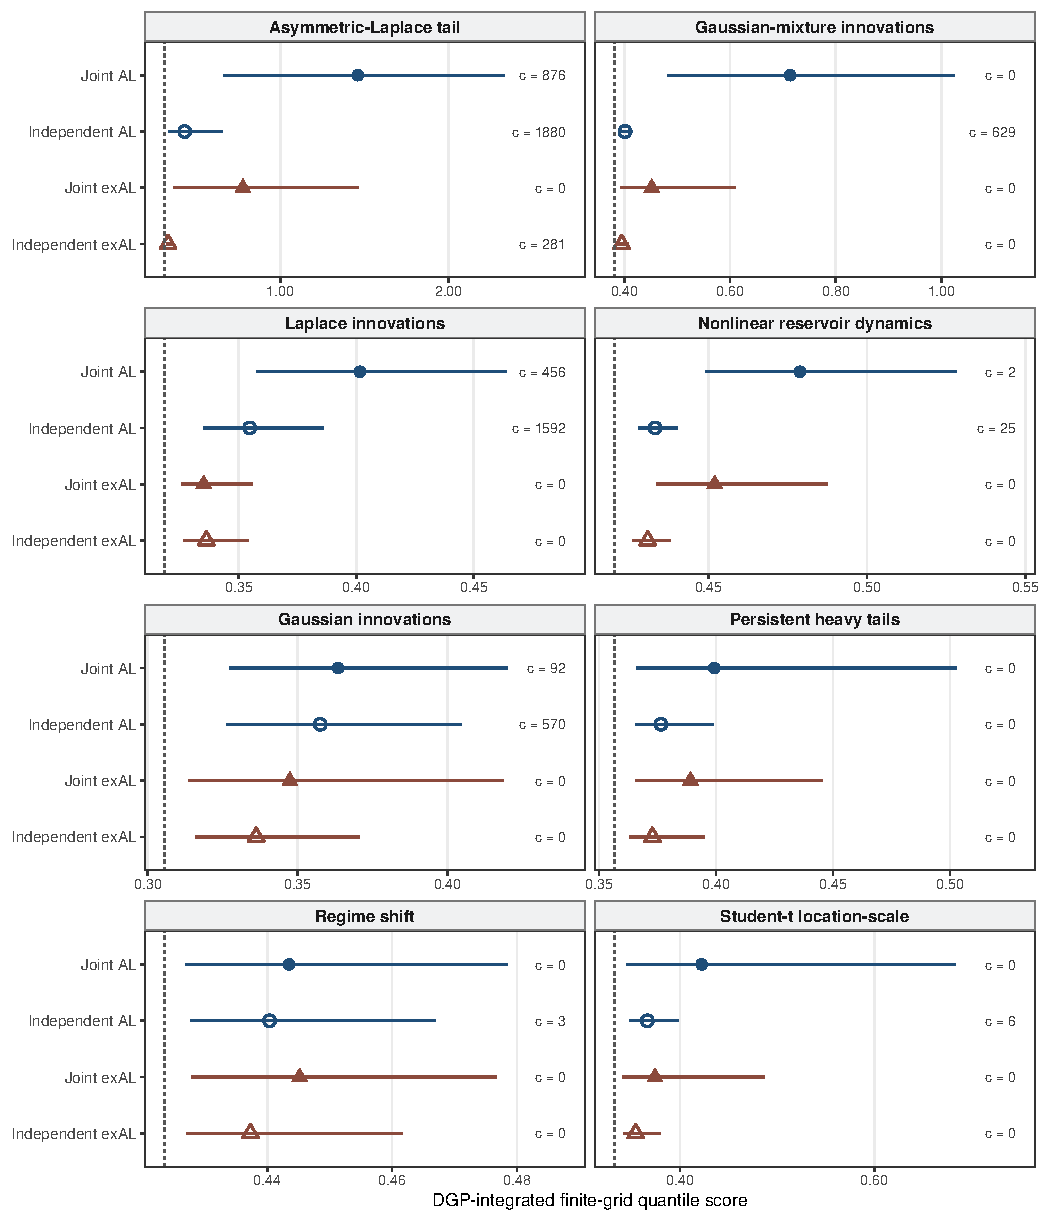
\includegraphics[width=0.94\textwidth]{figures/joint_qdesn_simulation/joint_qdesn_shared_backbone_forecast_dgp_score_intervals.pdf}
\caption{Posterior DGP-integrated finite-grid quantile scores under the shared-backbone design. Points are posterior means and horizontal bars are equal-tailed 95\% intervals; lower is better. Dashed lines mark the oracle finite-grid score. Filled symbols denote joint fits and open symbols independent fits; blue denotes \(\AL\) and red \(\exAL\). Labels \(c\) give raw crossings in the posterior-mean forecast grid; all counts after rearrangement are zero.}
\label{fig:joint-qdesn-shared-backbone-forecast-score}
\end{figure}
